\documentclass[11pt]{article}
\usepackage[a4paper,margin=1in]{geometry}
\usepackage[utf8]{inputenc}
\usepackage[T1]{fontenc}
\usepackage{amsmath,amssymb}
\usepackage{tikz}
\usetikzlibrary{trees,arrows.meta}
\usepackage[hidelinks]{hyperref}
\usepackage{booktabs}
\usepackage{enumitem}
\usepackage{array}

\title{Conditional Probability in Diagnostic Testing:\\
  An Isomorphism Between Tree Diagrams, Bayes' Theorem,\\
  Contingency Tables, and Likelihood Ratios,\\
  \large with the Clinical Risk Measures Read from the Same Table}
\author{Vasili Gavrilov\thanks{Independent researcher. ORCID 0009-0007-9371-5994. The author worked eleven years at a national Ministry of Health in a role unrelated to the topics of this paper. No funding; no competing interests.}}
\date{First version 29 May 2026; revised 6 September 2026}

\begin{document}
\maketitle

\begin{abstract}
\noindent Diagnostic test results are misread by patients and by clinicians, and the probability behind them is elementary. The same calculation circulates in four notations, each native to one profession: the tree diagram of statistics and decision analysis, Bayes' theorem of probability theory, the $2\times 2$ contingency table of epidemiology, and the odds and likelihood-ratio form of evidence-based medicine. The natural-frequency literature since Gigerenzer and Hoffrage (1995) has shown that the tree with counts on its leaves is the form people get right. It has not written the correspondence between the notations out. This paper does, on one worked example ($1\%$ prevalence, $80\%$ sensitivity, $9.6\%$ false-positive rate, positive predictive value $7.8\%$), row by row. It adds four things. First, the mapping itself, with the absolute and relative risk reduction (ARR, RRR) of trial reporting placed in the same table: they condition on the row, as sensitivity does, while the predictive value conditions on the column, and the paper says where that boundary lies. Second, a five-step Diagnostic Interpretation Procedure, whose first four steps are the natural-frequency method and whose fifth runs three checks, one for each documented failure mode: arithmetic error, base-rate neglect, and a relative figure taken for an absolute one. Third, a spreadsheet form of the procedure for sequences of tests, with a sum-to-one check after every step; on the running example, two conditionally independent positive results raise the posterior from $7.8\%$ to $41.2\%$, and a second test that repeats half of the first test's false positives raises it only to $13.2\%$. Fourth, the argument that medical and epidemiology curricula should teach every one of the notations, not the contingency table alone. The mathematics is classical; the contribution is the mapping, the procedure, and the curriculum argument.
\end{abstract}

\section{Introduction}

With the test of Section~\ref{sec:problem}, a positive result on a screening test at $1\%$ prevalence is a false alarm in 92 cases of 100. This follows from Bayes' theorem. Base-rate neglect goes back at least to Tversky and Kahneman (1974) \cite{tversky1974}. Casscells, Schoenberger, and Graboys (1978) \cite{casscells1978} gave 60 physicians and students a problem with a prevalence of 1 in 1{,}000 and a $5\%$ false-positive rate, sensitivity taken as perfect; the answer is under $2\%$, 11 gave it, and 27 answered $95\%$. Eddy (1982) \cite{eddy1982} catalogued the same errors, among them the confusion of $\Pr(D \mid T^+)$ with $\Pr(T^+ \mid D)$, later named the inverse fallacy \cite{villejoubert2002}. An informal Russian version of the present treatment appeared online in 2012 \cite{lj2012}.

Part of the persistence is notational. Each of the four notations of the abstract is read by one profession and by few others, and the calculation is one. Gigerenzer and Hoffrage (1995) \cite{gigerenzer1995} restated Bayesian problems in natural frequencies, the tree with absolute counts on its leaves, and correct answers among students rose from $16\%$ to $46\%$; Hoffrage and Gigerenzer (1998) \cite{hoffrage1998} found the same in physicians, and later work confirmed the effect for trees and $2\times 2$ tables \cite{binder2015, binder2018, binder2021, kunzelmann2022}. Gigerenzer et al.\ (2007) \cite{gigerenzer2007} treat ARR, RRR, and the number needed to treat beside natural frequencies. None of that literature writes the correspondence between the notations out. Section~\ref{sec:iso} gives the mapping, Section~\ref{sec:proc} the procedure and its spreadsheet form, Section~\ref{sec:disc} the curriculum argument.

\section{The Problem}
\label{sec:problem}

One worked example runs through the paper. It is the mammography problem of Eddy \cite{eddy1982} in the form used by Gigerenzer and Hoffrage \cite{gigerenzer1995}, kept so that the results below can be compared with that literature. Let
\begin{align*}
  \Pr(D) &= 0.01 && \text{prevalence in the screened population,}\\
  \Pr(T^+ \mid D) &= 0.80 && \text{sensitivity,}\\
  \Pr(T^+ \mid \neg D) &= 0.096 && \text{false-positive rate, } 1 - \text{specificity; specificity } 0.904.
\end{align*}
The clinic also uses ``false-positive rate'' for $1 - \mathrm{PPV}$, the share of positive results that are wrong; here it always means $1 - \text{specificity}$. The question is the positive predictive value $\mathrm{PPV} = \Pr(D \mid T^+)$, the probability that a person with a positive result has the disease. Intuition puts it near the sensitivity, $80\%$. It is $7.8\%$. We derive that value once per notation, then exhibit the correspondence.

\section{Four Notations}
\label{sec:four}

\subsection{Tree diagram}
\label{sec:tree}

Branch first on disease status, then on test result. Each edge carries a conditional probability; each leaf carries the product along its path.

\begin{center}
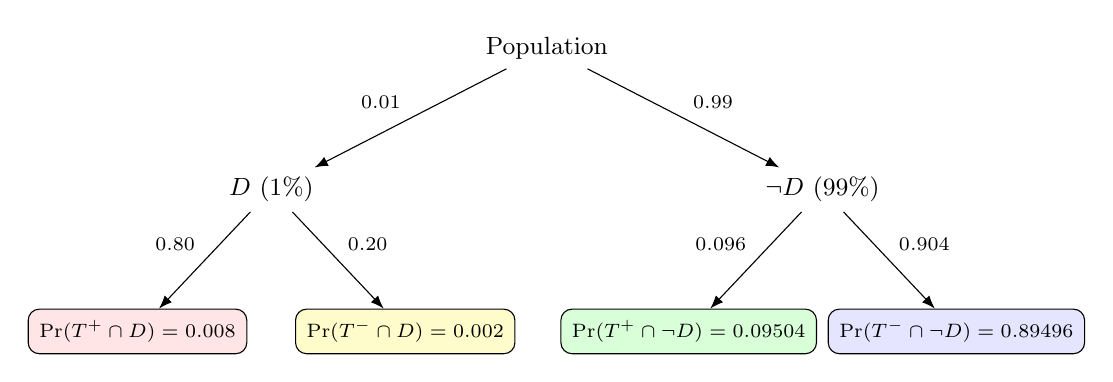
\begin{tikzpicture}[
  level distance=1.8cm,
  level 1/.style={sibling distance=7cm},
  level 2/.style={sibling distance=3.4cm},
  every node/.style={font=\small},
  edge from parent/.style={draw, -{Latex}},
  leaf/.style={draw, rounded corners, inner sep=4pt, font=\scriptsize}
]
\node {Population}
  child {
    node {$D$ ($1\%$)}
      child { node[leaf, fill=red!10]    {$\Pr(T^+ \cap D) = 0.008$}     edge from parent node[above left,  font=\scriptsize] {$0.80$} }
      child { node[leaf, fill=yellow!20] {$\Pr(T^- \cap D) = 0.002$}     edge from parent node[above right, font=\scriptsize] {$0.20$} }
    edge from parent node[above left, font=\scriptsize] {$0.01$}
  }
  child {
    node {$\neg D$ ($99\%$)}
      child { node[leaf, fill=green!15] {$\Pr(T^+ \cap \neg D) = 0.09504$} edge from parent node[above left,  font=\scriptsize] {$0.096$} }
      child { node[leaf, fill=blue!10]  {$\Pr(T^- \cap \neg D) = 0.89496$} edge from parent node[above right, font=\scriptsize] {$0.904$} }
    edge from parent node[above right, font=\scriptsize] {$0.99$}
  };
\end{tikzpicture}
\end{center}

Two leaves carry a positive result: the true positive $T^+ \cap D$ (red) and the false positive $T^+ \cap \neg D$ (green). The other two are excluded by the conditioning event. The PPV is the true-positive leaf over the sum of the positive leaves:
\begin{equation}
  \Pr(D \mid T^+) = \frac{0.008}{0.008 + 0.09504} = \frac{0.008}{0.10304} \approx 0.0776 \approx 7.8\%.
\end{equation}

The same four joint probabilities are the regions of a Venn diagram. The tree is read in sequence (first this, then that), the Venn by area (this region overlaps that one). The circle sizes below are not to scale, since a $1\%$ region is invisible at any readable size; the values are exact.

\begin{center}
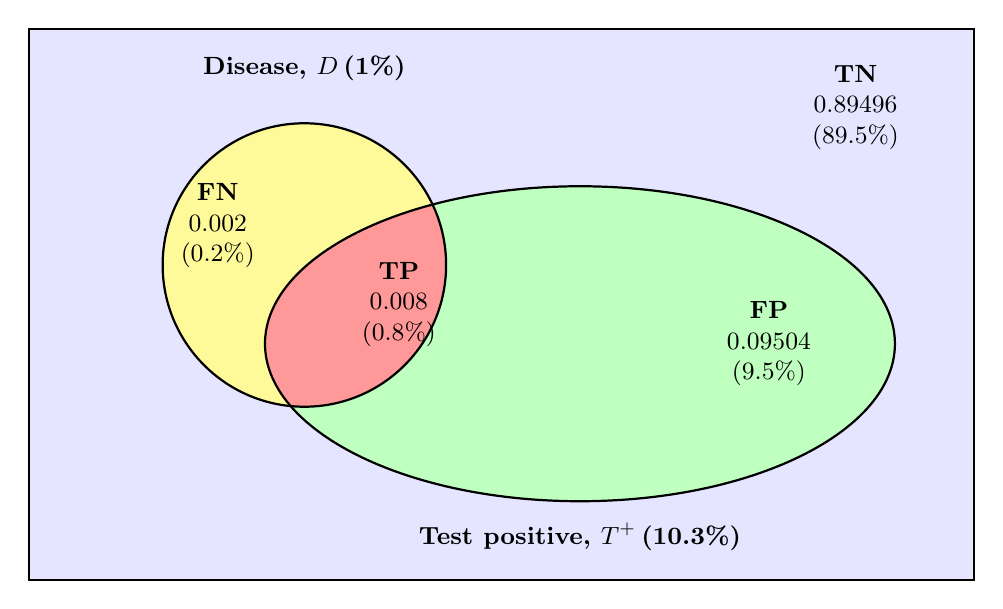
\begin{tikzpicture}[every node/.style={font=\small}]
  \fill[blue!10] (0,0) rectangle (12,7);
  \fill[green!25] (7,3) ellipse (4 and 2);
  \fill[yellow!40] (3.5,4) circle (1.8);
  \begin{scope}
    \clip (3.5,4) circle (1.8);
    \fill[red!40] (7,3) ellipse (4 and 2);
  \end{scope}
  \draw[thick] (0,0) rectangle (12,7);
  \draw[thick] (7,3) ellipse (4 and 2);
  \draw[thick] (3.5,4) circle (1.8);
  \node[align=center] at (2.4,4.5) {\textbf{FN}\\$0.002$\\$(0.2\%)$};
  \node[align=center] at (4.7,3.5) {\textbf{TP}\\$0.008$\\$(0.8\%)$};
  \node[align=center] at (9.4,3.0) {\textbf{FP}\\$0.09504$\\$(9.5\%)$};
  \node[align=center] at (10.5,6.0) {\textbf{TN}\\$0.89496$\\$(89.5\%)$};
  \node at (3.5,6.5) {\textbf{Disease, $D$\,(1\%)}};
  \node at (7.0,0.55) {\textbf{Test positive, $T^+$\,(10.3\%)}};
\end{tikzpicture}
\end{center}

The PPV is the red region over the whole ellipse: $0.8\% / 10.3\% \approx 7.8\%$.

\subsection{Bayes' theorem}

The same calculation, algebraically:\footnote{For the general theory rather than the diagnostic special case: Jaynes \cite{jaynes2003}, Sivia and Skilling \cite{sivia2006}, MacKay \cite{mackay2003}; Cox \cite{cox1946} for probability as an extension of logic; Gnedenko \cite{gnedenko1976} and Ventsel \cite{ventsel1965} for the Russian university and engineering traditions, both in English translation.}
\begin{align}
  \Pr(D \mid T^+) &= \frac{\Pr(T^+ \mid D)\,\Pr(D)}{\Pr(T^+ \mid D)\,\Pr(D) + \Pr(T^+ \mid \neg D)\,\Pr(\neg D)} \notag \\
  &= \frac{0.80 \times 0.01}{0.80 \times 0.01 + 0.096 \times 0.99} = \frac{0.008}{0.10304} \approx 7.8\%.
\end{align}
The numerator is the true-positive leaf. The denominator is the marginal probability of a positive test, the sum of the two positive leaves.

\subsection{Contingency table}
\label{sec:table}

Cross-classify a hypothetical population of $100{,}000$ against disease status and test result.

\begin{center}
\begin{tabular}{l|cc|c}
\toprule
                  & $T^+$    & $T^-$    & Row total \\
\midrule
$D$               & 800      & 200      & 1{,}000  \\
$\neg D$          & 9{,}504  & 89{,}496 & 99{,}000 \\
\midrule
Column total      & 10{,}304 & 89{,}696 & 100{,}000 \\
\bottomrule
\end{tabular}
\end{center}

Each interior cell is a leaf of the tree times the population size; the row totals are the first branching; the column totals are the marginals over the test result. The PPV is a cell over its column total:
\begin{equation}
  \Pr(D \mid T^+) = \frac{800}{10{,}304} \approx 7.8\%.
\end{equation}

The same four cells, drawn as quadrants, carry the vocabulary of hypothesis testing (Type I and II error) and of signal detection (hit, miss, false alarm, correct rejection). Readers from machine learning know the layout as the confusion matrix; programmers know it as two nested \texttt{if}/\texttt{else} conditions with four leaf states.

\begin{center}
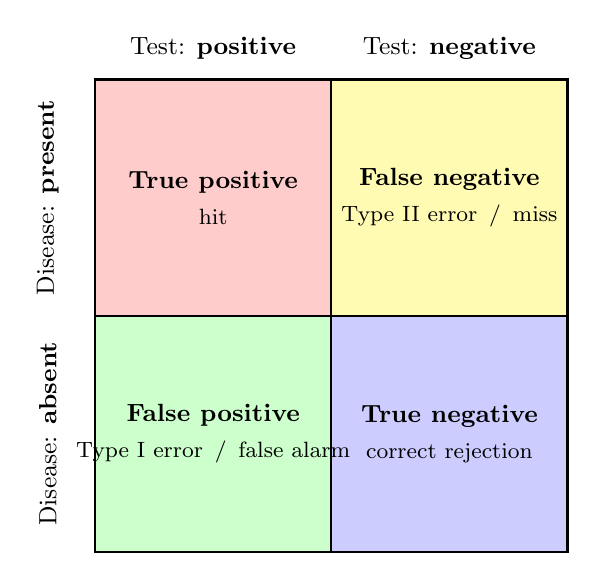
\begin{tikzpicture}[every node/.style={font=\small}]
  \fill[red!20]    (0,3) rectangle (3,6);
  \fill[yellow!30] (3,3) rectangle (6,6);
  \fill[green!20]  (0,0) rectangle (3,3);
  \fill[blue!20]   (3,0) rectangle (6,3);
  \draw[thick] (0,0) rectangle (6,6);
  \draw[thick] (3,0) -- (3,6);
  \draw[thick] (0,3) -- (6,3);
  \node[align=center] at (1.5, 4.5) {\textbf{True positive}\\[2pt]\footnotesize hit};
  \node[align=center] at (4.5, 4.5) {\textbf{False negative}\\[2pt]\footnotesize Type II error \,/\, miss};
  \node[align=center] at (1.5, 1.5) {\textbf{False positive}\\[2pt]\footnotesize Type I error \,/\, false alarm};
  \node[align=center] at (4.5, 1.5) {\textbf{True negative}\\[2pt]\footnotesize correct rejection};
  \node[font=\small] at (1.5, 6.4) {Test: \textbf{positive}};
  \node[font=\small] at (4.5, 6.4) {Test: \textbf{negative}};
  \node[font=\small, rotate=90] at (-0.6, 4.5) {Disease: \textbf{present}};
  \node[font=\small, rotate=90] at (-0.6, 1.5) {Disease: \textbf{absent}};
\end{tikzpicture}
\end{center}

The colours match the tree leaves. The diagonal holds the correct decisions, the off-diagonal the two error modes.

\subsection{Odds and likelihood ratios}
\label{sec:odds}

Evidence-based medicine writes the same calculation in odds. The likelihood ratio of a positive result is the ratio of the two positive edges of the tree, and it multiplies the prior odds:
\begin{align}
  \mathrm{LR}^+ &= \frac{\Pr(T^+ \mid D)}{\Pr(T^+ \mid \neg D)} = \frac{0.80}{0.096} \approx 8.33, &
  \mathrm{LR}^- &= \frac{\Pr(T^- \mid D)}{\Pr(T^- \mid \neg D)} = \frac{0.20}{0.904} \approx 0.221, \\
  \text{posterior odds} &= \frac{0.01}{0.99} \times 8.33 \approx 0.0842, &
  \mathrm{PPV} &= \frac{0.0842}{1 + 0.0842} \approx 7.8\%.
\end{align}
The Fagan nomogram of the bedside is this multiplication drawn on a ruler. The posterior odds are the ratio of the two positive leaves, $0.008 / 0.09504$, and of the two cells in the $T^+$ column, $800 / 9{,}504$.

\subsection{ARR and RRR}
\label{sec:arr}

Absolute and relative risk reduction compare two populations, a treatment arm and a control arm, rather than two states of one population, so they need a second example. Take a five-year primary-prevention trial with $10{,}000$ people per arm, $200$ events $E$ in the control arm and $50$ in the treatment arm:
\begin{align}
  \mathrm{ARR} &= \Pr(E \mid \text{control}) - \Pr(E \mid \text{treatment}) = 0.020 - 0.005 = 0.015 = 1.5\% \text{ over five years}, \\
  \mathrm{RRR} &= \frac{\Pr(E \mid \text{control}) - \Pr(E \mid \text{treatment})}{\Pr(E \mid \text{control})} = \frac{0.015}{0.020} = 75\%, \qquad
  \mathrm{NNT} = \frac{1}{\mathrm{ARR}} \approx 67.
\end{align}
The $2\times 2$ table is arm against outcome, both axes relabelled from the diagnostic table, and each risk is a cell over its row total. The same data give a $75\%$ RRR and a $1.5\%$ ARR; the gap is the lever of selective reporting. An ARR carries its time horizon or it means nothing, and the number needed to treat, NNT, is its reciprocal over the same horizon.

\section{The Isomorphism}
\label{sec:iso}

Each notation of Section~\ref{sec:four} presents the same object, the joint distribution on $\{D, \neg D\} \times \{T^+, T^-\}$, and marginalization and conditioning act identically in each; that is the sense of the word. The correspondence, row by row:

\begin{center}
\small
\renewcommand{\arraystretch}{1.25}
\begin{tabular}{p{0.16\textwidth}|p{0.15\textwidth}|p{0.24\textwidth}|p{0.15\textwidth}|p{0.07\textwidth}|p{0.07\textwidth}}
\toprule
\textbf{Concept}      & \textbf{Tree} & \textbf{Bayes term} & \textbf{Table} & \textbf{Value} & \textbf{Percent} \\
\midrule
True positive   & leaf $D \to T^+$    & $\Pr(T^+ \mid D)\,\Pr(D)$ & cell $D, T^+$ & 0.008 & 0.8\% \\
False negative  & leaf $D \to T^-$    & $\Pr(T^- \mid D)\,\Pr(D)$ & cell $D, T^-$ & 0.002 & 0.2\% \\
False positive  & leaf $\neg D \to T^+$ & $\Pr(T^+ \mid \neg D)\,\Pr(\neg D)$ & cell $\neg D, T^+$ & 0.09504 & 9.504\% \\
True negative   & leaf $\neg D \to T^-$ & $\Pr(T^- \mid \neg D)\,\Pr(\neg D)$ & cell $\neg D, T^-$ & 0.89496 & 89.496\% \\
\midrule
Marginal of $T^+$ & sum of the positive leaves & denominator & $T^+$ column total / $N$ & 0.10304 & 10.304\% \\
PPV, $\Pr(D \mid T^+)$ & true positive / positives & posterior & cell / column total & 0.0776 & 7.8\% \\
$\mathrm{LR}^+$ & ratio of the positive edges & $\Pr(T^+ \mid D)/\Pr(T^+ \mid \neg D)$ & row-conditional ratio & 8.33 & \\
Posterior odds & ratio of the positive leaves & numerator / second term & ratio within the $T^+$ column & 0.0842 & \\
\bottomrule
\end{tabular}
\end{center}

A practitioner who holds this table can read a paper written in any of the four.

The risk measures of Section~\ref{sec:arr} live in the same table with the axes relabelled, and they condition on the row:

\begin{center}
\renewcommand{\arraystretch}{1.25}
\begin{tabular}{p{0.17\textwidth}|p{0.17\textwidth}|p{0.22\textwidth}|p{0.17\textwidth}|p{0.08\textwidth}}
\toprule
\textbf{Concept} & \textbf{Tree} & \textbf{Bayes term} & \textbf{Table} & \textbf{Value} \\
\midrule
Control risk   & edge control $\to E$   & $\Pr(E \mid \text{control})$   & cell / row total & 2.0\% \\
Treatment risk & edge treatment $\to E$ & $\Pr(E \mid \text{treatment})$ & cell / row total & 0.5\% \\
ARR & difference of the two edges & $\Pr(E \mid \text{c}) - \Pr(E \mid \text{t})$ & difference of row-conditionals & 1.5\% \\
RRR & that difference over the control edge & $\mathrm{ARR} / \Pr(E \mid \text{c})$ & same, over the control row & 75\% \\
\bottomrule
\end{tabular}
\end{center}

Row conditioning is the direction of sensitivity and the false-positive rate, not of PPV. The counterpart of ARR in the diagnostic table is Youden's index, $\text{sensitivity} - \text{false-positive rate} = 0.80 - 0.096 = 0.704$, and the counterpart of RRR is that index over the sensitivity, $0.88$; PPV, the column-conditional quantity, has no counterpart in a trial table. A reader who is told that PPV and ARR are one calculation will conflate them; they are two conditionings of one table.

\section{A Diagnostic Interpretation Procedure}
\label{sec:proc}

The failure is procedural. The procedure below is for a clinician, epidemiologist, journalist, or patient facing a test result or a trial finding. Steps 1--4 are the natural-frequency method \cite{gigerenzer1995, hoffrage1998}; step 5 is this paper's addition.

\begin{enumerate}[leftmargin=2em,itemsep=0.4em]
  \item \textbf{Find the pretest probability.} For a screening programme, the detection rate per round in the invited age band, from the programme's own report. For a patient with a presentation, the pretest probability for that presentation from a validated prediction rule or a local audit, not the population prevalence. For a trial, the control-arm event rate from the primary outcome table of the primary publication. If the source gives only a relative measure and no base rate, stop: the figure cannot be interpreted.
  \item \textbf{Convert every rate to counts in a fixed population.} Choose $N$ so that the smallest cell holds at least 10 people: $10{,}000$ for a $1\%$ condition, $100{,}000$ for $0.1\%$. Multiply each rate by $N$.
  \item \textbf{Fill the $2\times 2$ table of counts.} Four cells: disease and positive, disease and negative, no disease and positive, no disease and negative.
  \item \textbf{Compute the answer from the counts, not from a relative summary.} PPV is the disease-and-positive cell over the positive column total, or post-test odds $=$ pretest odds $\times \mathrm{LR}^+$; the two agree. ARR is the control-arm event count over the control-arm size minus the treatment-arm event count over the treatment-arm size. RRR is ARR over the control-arm rate; NNT is $1/\mathrm{ARR}$.
  \item \textbf{Run three checks before accepting the answer.}
  \begin{enumerate}[label=(\alph*),leftmargin=2em,itemsep=0.2em]
    \item \emph{Sum check.} The four cells sum to $N$; otherwise there is an arithmetic error.
    \item \emph{Base-rate check.} Compute $\mathrm{LR}^+ = \text{sensitivity} / \text{false-positive rate}$. For any test with $\mathrm{LR}^+ \geq 1$ the PPV cannot exceed $\text{prevalence} \times \mathrm{LR}^+$. When that bound is small, a PPV near the sensitivity is base-rate neglect; when the bound is near or above $1$, a high PPV is legitimate, as it is for a confirmatory test with a $0.1\%$ false-positive rate.
    \item \emph{Absolute-against-relative check.} Never accept an RRR without the ARR and NNT beside it, over a stated horizon. The ratio $\mathrm{RRR}/\mathrm{ARR}$ equals $1 / \Pr(E \mid \text{control})$: a large ratio is a low baseline risk, which is when the relative figure misleads on its own.
  \end{enumerate}
\end{enumerate}

\paragraph{The running example.}
Base rate $1\%$; $N = 10{,}000$. Then $100$ have the disease, of whom $80$ test positive and $20$ negative; $9{,}900$ do not, of whom $950$ test positive ($9{,}900 \times 0.096 = 950.4$, rounded) and $8{,}950$ negative. $\mathrm{PPV} = 80/(80+950) = 80/1{,}030 \approx 7.8\%$. Checks: (a) $80 + 20 + 950 + 8{,}950 = 10{,}000$; (b) $0.01 \times 8.33 = 0.083$, and $7.8\%$ is below it; (c) no relative measure was reported. Accepted. Section~\ref{sec:table} used $N = 100{,}000$ and got $9{,}504$ false positives; the rounding here changes no ratio at the precision shown. A reader can run the three checks without an external authority.

\subsection*{Spreadsheet form for sequences of tests}

When there is more than one test (screen then confirmation, longitudinal monitoring, tests of different modality), the procedure takes a flat spreadsheet form. Each row is one path of outcomes; each column from left to right is one step; the rightmost column is the joint probability of the path, rounded to five places. After every step the rightmost column must sum to $1$. That is the renormalization check at that depth.

Suppose the test of Section~\ref{sec:problem} is applied to the same patient twice, and assume for the moment that the two outcomes are conditionally independent given disease status. The assumption is a teaching device: two runs of one test on one specimen or platform share error sources (specimen quality, calibration drift, operator, biological confounders) and are positively correlated. When it fails, the columns hold $\Pr(T_2 \mid T_1, D)$ and $\Pr(T_2 \mid T_1, \neg D)$ in place of $\Pr(T_2 \mid D)$ and $\Pr(T_2 \mid \neg D)$. The shape of the spreadsheet does not change. The assumption is most defensible when the tests differ in analyte or mechanism, a serological screen followed by a nucleic-acid confirmation, say, so that the error sources are distinct.

\paragraph{Step 0, the prior.} Two rows, one per disease status.

\begin{center}
\renewcommand{\arraystretch}{1.15}
\begin{tabular}{c|c|l}
\toprule
\textbf{Row} & \textbf{Disease} & \textbf{Joint probability after step 0} \\
\midrule
1 & $D$      & $0.01$ \\
2 & $\neg D$ & $0.99$ \\
\midrule
  & \multicolumn{1}{r|}{\textbf{Sum}} & $\;\;\mathbf{1.00000}$ \\
\bottomrule
\end{tabular}
\end{center}

\paragraph{Step 1, after test 1.} Each row splits in two, one per outcome; the new joint is the old joint times the conditional probability of the outcome.

\begin{center}
\renewcommand{\arraystretch}{1.15}
\begin{tabular}{c|c|c|l}
\toprule
\textbf{Row} & \textbf{Disease} & \textbf{Test 1} & \textbf{Joint probability after step 1} \\
\midrule
1 & $D$      & $+$ & $0.01 \times 0.80 = 0.00800$ \\
2 & $D$      & $-$ & $0.01 \times 0.20 = 0.00200$ \\
3 & $\neg D$ & $+$ & $0.99 \times 0.096 = 0.09504$ \\
4 & $\neg D$ & $-$ & $0.99 \times 0.904 = 0.89496$ \\
\midrule
  & \multicolumn{2}{r|}{\textbf{Sum}} & $\;\;\mathbf{1.00000}$ \\
\bottomrule
\end{tabular}
\end{center}

\paragraph{Step 2, after test 2.} Each row splits again.

\begin{center}
\renewcommand{\arraystretch}{1.15}
\begin{tabular}{c|c|c|c|l}
\toprule
\textbf{Row} & \textbf{Disease} & \textbf{Test 1} & \textbf{Test 2} & \textbf{Joint probability after step 2} \\
\midrule
1 & $D$      & $+$ & $+$ & $0.00800 \times 0.80   \approx 0.00640$ \\
2 & $D$      & $+$ & $-$ & $0.00800 \times 0.20   \approx 0.00160$ \\
3 & $D$      & $-$ & $+$ & $0.00200 \times 0.80   \approx 0.00160$ \\
4 & $D$      & $-$ & $-$ & $0.00200 \times 0.20   \approx 0.00040$ \\
5 & $\neg D$ & $+$ & $+$ & $0.09504 \times 0.096  \approx 0.00912$ \\
6 & $\neg D$ & $+$ & $-$ & $0.09504 \times 0.904  \approx 0.08592$ \\
7 & $\neg D$ & $-$ & $+$ & $0.89496 \times 0.096  \approx 0.08592$ \\
8 & $\neg D$ & $-$ & $-$ & $0.89496 \times 0.904  \approx 0.80904$ \\
\midrule
  & \multicolumn{3}{r|}{\textbf{Sum}} & $\;\;\mathbf{1.00000}$ \\
\bottomrule
\end{tabular}
\end{center}

After $n$ tests the table has $2^{n+1}$ rows.

\paragraph{Reading off a posterior.} Filter the rows on the observed outcomes; sum the matching joints for $D$; divide by the sum of all matching joints. After two positive results the matching rows are 1 and 5:
\begin{equation*}
  \Pr(D \mid T_1^+ \cap T_2^+) = \frac{0.00640}{0.00640 + 0.00912} = \frac{0.00640}{0.01552} \approx 41.2\%.
\end{equation*}
In this example the second result moves the posterior from $7.8\%$ into the range where the next, more invasive, diagnostic step is justified; the treatment threshold is set per disease from the costs of the two errors.

\paragraph{The pruned form.} The clinic observes one path, so at each step it needs only two rows: the posterior of the previous step as the prior of the next. After $T_1^+$ the rows are $D$: $0.0776$ and $\neg D$: $0.9224$. Multiplying by test 2 gives $0.0776 \times 0.80 = 0.0621$ and $0.9224 \times 0.096 = 0.0886$, and $0.0621 / (0.0621 + 0.0886) = 41.2\%$, as before. The full table is the audit version; the two-row table is the working version.

\paragraph{When the tests disagree.} Suppose $T_1$ positive and $T_2$ negative, still under independence. Rows 2 and 6:
\begin{equation*}
  \Pr(D \mid T_1^+ \cap T_2^-) = \frac{0.00160}{0.00160 + 0.08592} \approx 1.8\%.
\end{equation*}
The posterior is back near the prior of $1\%$. In odds: the positive multiplies the prior odds by $\mathrm{LR}^+ \approx 8.3$, the negative by $\mathrm{LR}^- \approx 0.22$, and the product is $1.8$, so the odds barely move. Any other combination of outcomes is one filter on the same table.

\paragraph{When the tests are correlated.} Suppose the second test repeats half of the first test's false positives, and
\begin{align*}
  \Pr(T_2^+ \mid T_1^+, D)      &= 0.90, & \Pr(T_2^+ \mid T_1^-, D)      &= 0.40, \\
  \Pr(T_2^+ \mid T_1^+, \neg D) &= 0.50, & \Pr(T_2^+ \mid T_1^-, \neg D) &= 0.053.
\end{align*}
These values keep the marginals of $T_2$ equal to those of $T_1$: $0.80 \times 0.90 + 0.20 \times 0.40 = 0.80$ and $0.096 \times 0.50 + 0.904 \times 0.053 \approx 0.096$, so what changes between this case and the last is the correlation alone. They are illustrative; such conditionals come only from latent-class estimates with conditional dependence, not from a test's package insert. The two rows that matter become
\begin{align*}
  \Pr(D, T_1^+, T_2^+)      &= 0.01 \times 0.80 \times 0.90 = 0.00720, \\
  \Pr(\neg D, T_1^+, T_2^+) &= 0.99 \times 0.096 \times 0.50 = 0.04752,
\end{align*}
and
\begin{equation*}
  \Pr(D \mid T_1^+ \cap T_2^+) = \frac{0.00720}{0.00720 + 0.04752} \approx 13.2\%.
\end{equation*}
Confirmation should therefore use a test whose error sources are independent of the screen's and whose specificity is high; a different analyte or mechanism usually gives both. Repeating the same test is informative only where its error is random rather than intrinsic to the patient.

Excel and Google Sheets hold this layout as it stands, and a reviewer can recompute every cell. The five steps apply to the spreadsheet row by row.

\section{Discussion}
\label{sec:disc}

\subsection{Why the misreading persists}

One cause is visible in the notations themselves. ARR and RRR reach the reader as summary statistics without the table that produced them, and a reader given ``$95\%$ relative risk reduction'' has no way back to the absolute scale. The RRR discards that scale; the table and the tree keep it in the counts; the formula shows it only after substitution. Kahwati et al.\ (2017) \cite{kahwati2017}, reviewing studies of prescribers, found that the same result presented as a relative rather than an absolute reduction raises the perceived effectiveness of a treatment and the willingness to prescribe it.

Brown (2021) \cite{brown2021} and Olliaro et al.\ (2021) \cite{olliaro2021} recompute the COVID-19 mRNA vaccine trials both ways. The trial publications reported the case counts; what reached the public were the relative reductions of $94$--$95\%$, while the absolute reductions over the trial follow-up of about two months were $0.7$--$1.2\%$, depending on the denominator, with a number needed to vaccinate near $100$. Both figures are correct and answer different questions: the relative figure transports to other attack rates, the absolute figure belongs to two months at the trial's incidence and grows with exposure.

\subsection{Recommendations}

For reporting: the counts. Primary reports are held to this by STARD 2015, item 23 \cite{bossuyt2015}, and CONSORT 2010, item 17b \cite{schulz2010}, and largely comply; the counts drop out in abstracts, press releases, advertising, and public statements. The recommendation is that the $2\times 2$ table of absolute counts travel with every derived statistic (PPV, ARR, RRR, sensitivity, specificity, likelihood ratio) into those channels. A tree of four leaves adds the conditional structure and takes a quarter of a page.

For training: epidemiology and clinical curricula introduce conditional probability through the contingency table and its derived statistics. The table is complete and concise, and it makes one thing salient, the joint frequency of each cell. The conditional flow from prior to posterior is salient in the tree, the algebraic identity in the formula, the update as a multiplication in the odds form, and the absolute scale in the tree and the table. The natural-frequency studies \cite{gigerenzer1995, hoffrage1998, binder2015, binder2018, binder2021, kunzelmann2022} put the gain from the tree and the counts at about 30 percentage points of correct answers. Medical, epidemiology, and public-health curricula and prescribers' continuing education should cover every notation of Section~\ref{sec:four} through the mapping of Section~\ref{sec:iso} and the procedure of Section~\ref{sec:proc}. The cost is a few hours in the existing biostatistics block.

\subsection{Iterated inference}

Under repeated observation the posterior of one step is the prior of the next, as in Bayesian networks \cite{pearl1988} and hidden Markov models. The notations of Section~\ref{sec:four} apply to each update, and the pruned spreadsheet of Section~\ref{sec:proc} is that iteration written out.

\subsection{Limitations}

\begin{itemize}[leftmargin=1.5em,itemsep=0.2em]
  \item \emph{Binary outcomes.} The examples assume binary disease status and binary test results. The mapping extends to graded severity, competing diagnoses, and ordinal scores, with correspondingly larger tables, trees, and spreadsheets; the paper does not work that out.
  \item \emph{Step 5 is untested.} The three checks have not been evaluated on students or clinicians.
  \item \emph{Scope of the cited evidence.} Casscells et al.\ and Kahwati et al.\ document misreading by individual clinicians; Brown and Olliaro et al.\ document reporting in specific trials. That these patterns carry into regulatory and public communication is consistent with the evidence and not established by it.
\end{itemize}

\section*{Acknowledgements}

The author thanks Anna Martirosyan for discussions of absolute and relative risk reduction, which started this work, and Elena Vasserman for discussions of the epidemiological context.

\begin{thebibliography}{99}

\bibitem{tversky1974}
A.\ Tversky and D.\ Kahneman,
``Judgment under Uncertainty: Heuristics and Biases,''
\emph{Science}, vol.\ 185, no.\ 4157, pp.\ 1124--1131, 1974.

\bibitem{gigerenzer1995}
G.\ Gigerenzer and U.\ Hoffrage,
``How to Improve Bayesian Reasoning Without Instruction: Frequency Formats,''
\emph{Psychological Review}, vol.\ 102, no.\ 4, pp.\ 684--704, 1995.

\bibitem{hoffrage1998}
U.\ Hoffrage and G.\ Gigerenzer,
``Using Natural Frequencies to Improve Diagnostic Inferences,''
\emph{Academic Medicine}, vol.\ 73, no.\ 5, pp.\ 538--540, 1998.

\bibitem{binder2015}
K.\ Binder, S.\ Krauss, and G.\ Bruckmaier,
``Effects of visualizing statistical information: An empirical study on tree diagrams and $2\times 2$ tables,''
\emph{Frontiers in Psychology}, vol.\ 6, article 1186, 2015.
\url{https://www.ncbi.nlm.nih.gov/pmc/articles/PMC4549558/}

\bibitem{binder2018}
K.\ Binder, S.\ Krauss, G.\ Bruckmaier, and J.\ Marienhagen,
``Visualizing the Bayesian 2-test case: The effect of tree diagrams on medical decision making,''
\emph{PLOS ONE}, vol.\ 13, no.\ 3, e0195029, 2018.
\url{https://journals.plos.org/plosone/article?id=10.1371/journal.pone.0195029}

\bibitem{binder2021}
K.\ Binder, S.\ Krauss, R.\ Schmidmaier, and L.\ T.\ Braun,
``Natural frequency trees improve diagnostic efficiency in Bayesian reasoning,''
\emph{Advances in Health Sciences Education}, vol.\ 26, no.\ 3, pp.\ 847--863, 2021.
\url{https://link.springer.com/article/10.1007/s10459-020-10025-8}

\bibitem{kunzelmann2022}
A.\ K.\ Kunzelmann, K.\ Binder, M.\ R.\ Fischer, M.\ Reincke, L.\ T.\ Braun, and R.\ Schmidmaier,
``Improving Diagnostic Efficiency with Frequency Double-Trees and Frequency Nets in Bayesian Reasoning,''
\emph{MDM Policy \& Practice}, vol.\ 7, no.\ 1, 2022.
\url{https://pmc.ncbi.nlm.nih.gov/articles/PMC8935422/}

\bibitem{gigerenzer2007}
G.\ Gigerenzer, W.\ Gaissmaier, E.\ Kurz-Milcke, L.\ M.\ Schwartz, and S.\ Woloshin,
``Helping Doctors and Patients Make Sense of Health Statistics,''
\emph{Psychological Science in the Public Interest}, vol.\ 8, no.\ 2, pp.\ 53--96, 2007.

\bibitem{casscells1978}
W.\ Casscells, A.\ Schoenberger, and T.\ B.\ Graboys,
``Interpretation by Physicians of Clinical Laboratory Results,''
\emph{New England Journal of Medicine}, vol.\ 299, no.\ 18, pp.\ 999--1001, 1978.

\bibitem{eddy1982}
D.\ M.\ Eddy,
``Probabilistic Reasoning in Clinical Medicine: Problems and Opportunities,''
in D.\ Kahneman, P.\ Slovic, and A.\ Tversky (eds.),
\emph{Judgment Under Uncertainty: Heuristics and Biases},
Cambridge University Press, 1982, pp.\ 249--267.

\bibitem{villejoubert2002}
G.\ Villejoubert and D.\ R.\ Mandel,
``The inverse fallacy: An account of deviations from Bayes's theorem and the additivity principle,''
\emph{Memory \& Cognition}, vol.\ 30, no.\ 2, pp.\ 171--178, 2002.

\bibitem{pearl1988}
J.\ Pearl,
\emph{Probabilistic Reasoning in Intelligent Systems: Networks of Plausible Inference},
Morgan Kaufmann, San Mateo, CA, 1988.

\bibitem{jaynes2003}
E.\ T.\ Jaynes,
\emph{Probability Theory: The Logic of Science},
Cambridge University Press, 2003.

\bibitem{sivia2006}
D.\ S.\ Sivia and J.\ Skilling,
\emph{Data Analysis: A Bayesian Tutorial}, 2nd ed.,
Oxford University Press, 2006.

\bibitem{mackay2003}
D.\ J.\ C.\ MacKay,
\emph{Information Theory, Inference, and Learning Algorithms},
Cambridge University Press, 2003.
\url{http://www.inference.org.uk/itila/}

\bibitem{cox1946}
R.\ T.\ Cox,
``Probability, Frequency and Reasonable Expectation,''
\emph{American Journal of Physics}, vol.\ 14, no.\ 1, pp.\ 1--13, 1946.

\bibitem{kahwati2017}
L.\ Kahwati, D.\ Carmody, N.\ Berkman, H.\ Sullivan, K.\ Aikin, and J.\ DeFrank,
``Prescribers' Knowledge and Skills for Interpreting Research Results: A Systematic Review,''
\emph{Journal of Continuing Education in the Health Professions}, vol.\ 37, no.\ 2, pp.\ 129--136, 2017.
\url{https://pmc.ncbi.nlm.nih.gov/articles/PMC8218608/}

\bibitem{brown2021}
R.\ B.\ Brown,
``Outcome Reporting Bias in COVID-19 mRNA Vaccine Clinical Trials,''
\emph{Medicina (Kaunas)}, vol.\ 57, no.\ 3, article 199, 2021.
\url{https://pmc.ncbi.nlm.nih.gov/articles/PMC7996517/}

\bibitem{olliaro2021}
P.\ Olliaro, E.\ Torreele, and M.\ Vaillant,
``COVID-19 vaccine efficacy and effectiveness: the elephant (not) in the room,''
\emph{The Lancet Microbe}, vol.\ 2, no.\ 7, pp.\ e279--e280, 2021.
\url{https://pmc.ncbi.nlm.nih.gov/articles/PMC8057721/}

\bibitem{bossuyt2015}
P.\ M.\ Bossuyt, J.\ B.\ Reitsma, D.\ E.\ Bruns, et al.,
``STARD 2015: an updated list of essential items for reporting diagnostic accuracy studies,''
\emph{BMJ}, vol.\ 351, h5527, 2015.

\bibitem{schulz2010}
K.\ F.\ Schulz, D.\ G.\ Altman, and D.\ Moher,
``CONSORT 2010 Statement: updated guidelines for reporting parallel group randomised trials,''
\emph{BMJ}, vol.\ 340, c332, 2010.

\bibitem{gnedenko1976}
B.\ V.\ Gnedenko,
\emph{The Theory of Probability},
trans.\ from Russian, Mir Publishers, Moscow, 1976.

\bibitem{ventsel1965}
E.\ S.\ Ventsel (Wentzel),
\emph{Probability Theory},
trans.\ from Russian, Mir Publishers, Moscow, 1965.

\bibitem{lj2012}
V.\ Gavrilov,
``Solving Conditional Probability Problems for Schoolchildren'' (in Russian),
online article, 25 April 2012.

\end{thebibliography}

\end{document}
